\section{Cartograms with Dynamic Features}

{
\begin{figure}[b!]
    \centering
    \includegraphics[width=\columnwidth]{example-image-a}
    \caption{An overview of \software. Figure TBA.}
    \label{fig:overview}
\end{figure}
}

\algoref{alg:UpdateNodePosition} provides an overview of our algorithm. We first load and render the CCG geospatial boundaries. For each CCG we compute the centroid and represent it using a square node with $ s $ as its size. We then apply the Fast Node Overlap Removal (VPSC) algorithm \cite{dwyer2006fast} repeatedly to remove overlaps. We chose VPSC over other node overlap removal algorithms since VPSC is able to provide spread minimization and node movement minimization while maintaining a good level of global shape preservation \cite{chen2020Node}. During each iteration, we compute node trajectories (See \algoref{alg:check river crossing}) and translate nodes to their new position. Nodes that cross a river are translated back to their previous position. This procedure ends when 1) no overlaps are present; 2) no nodes cross a river. We then increase $ \nodeSize $ by one pixel and repeat the algorithm until the max node size $ \nodeSizeMax $ is reached.

% \begin{noindent}

\begin{algorithm}[tb!]
    \caption{Procedure to update node positions by removing overlap and prevent nodes from crossing rivers.}\label{alg:UpdateNodePosition}
    \textbf{Global variables:} \\
    $ \nodeList \gets $ a list of nodes representing CCGs \\
    $ \nodeSize \gets $ the current size of all nodes \\
    $ \nodeSizeMax \gets $ the maximum size of a node \\
    $ \stalemate \gets $ the maximum number of iterations indicating a stalemate \\

    \textbf{Local variables:} \\
    $ \nodeListVPSC \gets $ a list of nodes representing CCGs after running VPSC \\
    $ \crossRiver \gets $ boolean indicating a node crossed a river \\

    \begin{algorithmic}[1]
        \Procedure{UpdateNodePosition}{}
        \While{$ \nodeSize < \nodeSizeMax $}

        \State $ \nodeListVPSC \gets $ RunVPSC ($ \nodeList $)

            \ForEach {$ \nodeListVPSCEach \in \nodeListVPSC $}

                \If {TranslateNode ($ \nodeListEach, \nodeListVPSCEach $)}
                    \State $ \crossRiver \gets $ \Call{TestRiverCross}{$ \nodeListEach, \nodeListVPSCEach $}

                    \If{$ \crossRiver = True $}
                        \State $ \stalemate \gets \stalemate + 1 $

                        \If{$ \stalemate < \stalemate $}
                            \State \Call{TranslateNode}{$ \nodeListEach $}
                        \Else
                            \State \Call{DeriveCorridor}{$ \nodeListEach, \nodeListVPSCEach $}
                        \EndIf

                    \EndIf

                \EndIf

            \EndFor

        \EndWhile

        \State $ \nodeSize \gets \nodeSize ++$

        \EndProcedure
    \end{algorithmic}
\end{algorithm}


\begin{algorithm}[tb!]
    \caption{Procedure to update a single node, $ \node $'s position.}\label{alg:move position}

    \textbf{Input:} \\
    $ \node \gets $ required, the node \\
    $ \nodeVPSC \gets $ optional, the node after running VPSC \\

    \textbf{Output:} \\
    A boolean for whether the node's position is updated. \\

    \begin{algorithmic}[1]
        \Procedure{TranslateNode}{$ \node, \nodeVPSC $}
        \If{$ \node.x = \nodeVPSC.x $ and $ \node.y = \nodeVPSC.y $}
            \item[] \Comment{Node position remains unchanged}
            \State \Return{$ False $}
        \EndIf

        \If{$ \nodeVPSC$ is undefined } 
        \item[] \Comment{When optional parameter $ \nodeVPSC $ is undefined}
        \item[] \Comment{Move the node back to its previous position}
            \State $ \node.x \gets \node.previous.x,~\node.y \gets \node.previous.y $
        \Else
            \State $ \node.x \gets \nodeVPSC.x,~\node.y \gets \nodeVPSC.y $
            \State $ \node.history.push(\node.x, \node.y) $
        \EndIf
        \State \Return{$ True $}
        \EndProcedure
    \end{algorithmic}
\end{algorithm}

%\end{noindent}

\subsection{River Cross Testing}

We use rivers as topological boundaries and prevent nodes from crossing them. When a node's position changes, we test if the node's trajectory intersects any segment of a river. See \algoref{alg:check river crossing}. A bounding box intersection test can be performed to reduce the number of edge intersection detections required.

% \begin{noindent}
\begin{algorithm}[tb!]
    \caption{Procedure to test if a node crosses a river.}\label{alg:check river crossing}
    \textbf{Input:} \\
    $ \node \gets $ required, the node \\
    $ \nodeVPSC \gets $ required, the node after running VPSC \\

    \textbf{Output:} \\
    A boolean indicating the node crosses a river. \\

    \textbf{Global variables:} \\
    $ \riverEdgeList \gets $ a list of river edges \\

    \textbf{Local variables:} \\
    $ \riverEdgeListEach \gets $ a river edge in $ \riverEdgeList $ \\ 
    $ \nodeBoundingBox, \riverEdgeBoundingBoxEach \gets $ the bounding boxes for $ \node $ and $ \riverEdgeListEach $ \\
    $ \boundingBoxInt \gets $ boolean indicating $ \nodeBoundingBox $ intersects $ \riverEdgeBoundingBoxEach $ \\
    $ \nodeEdge \gets $ the edge for $ \node $\\
    $ \edgeBoxInt \gets $ boolean indicating $ \nodeEdge $ intersects $ \riverEdgeListEach $ \\

    \begin{algorithmic}[1]
        \Procedure{TestRiverCross}{$ \node, \nodeVPSC $}
        
        \ForEach{$ \riverEdgeListEach \in \riverEdgeList $}
            \State $ \nodeBoundingBox \gets $ GenerateBoundingBox ($ \node, \nodeVPSC $)
            \State $ \riverEdgeBoundingBoxEach \gets $ GenerateBoundingBox ($ \riverEdgeListEach $)
            \State $ \boundingBoxInt \gets $ TestBoundingIntersection ($ \nodeBoundingBox, \riverEdgeBoundingBoxEach $)
            
            \If{$ \boundingBoxInt = True $}
                \State $ e_{n} \gets $ GenerateEdge ($ \node, \nodeVPSC $)
                \State $ \edgeBoxInt \gets $ TestEdgeIntersection ($ \nodeEdge, \riverEdgeListEach $)
                
                \If{$ \edgeBoxInt = True $}
                    \State \Return{$ True $}
                \EndIf
            
                \EndIf
        \EndFor
        
        \State \Return{$ False $}
        \EndProcedure
    \end{algorithmic}
\end{algorithm}
%\end{noindent}

\subsection{Corridor Derivation}

As the VPSC always tries to produce an optimal node layout where node distribution and translation are minimized, a node might be repeatedly translated between two positions due to river crossing and congestion, creating a stalemate situation, as shown in \figref{fig:stalemate}. In order to create space for VPSC to generate a new layout, we introduce a parameter, $ \stalemate $, to test for stalemate. If a node is translated between two positions for more than $ \stalemate $ iterations, it is considered to be in a stalemate. A stalemate triggers a corridor derivation which moves all nodes within the corridor by $ d $ set by the user (See \figref{fig:corridor} and \algoref{alg:derive corridor}).

{
\begin{figure}[tb!]
    \centering
    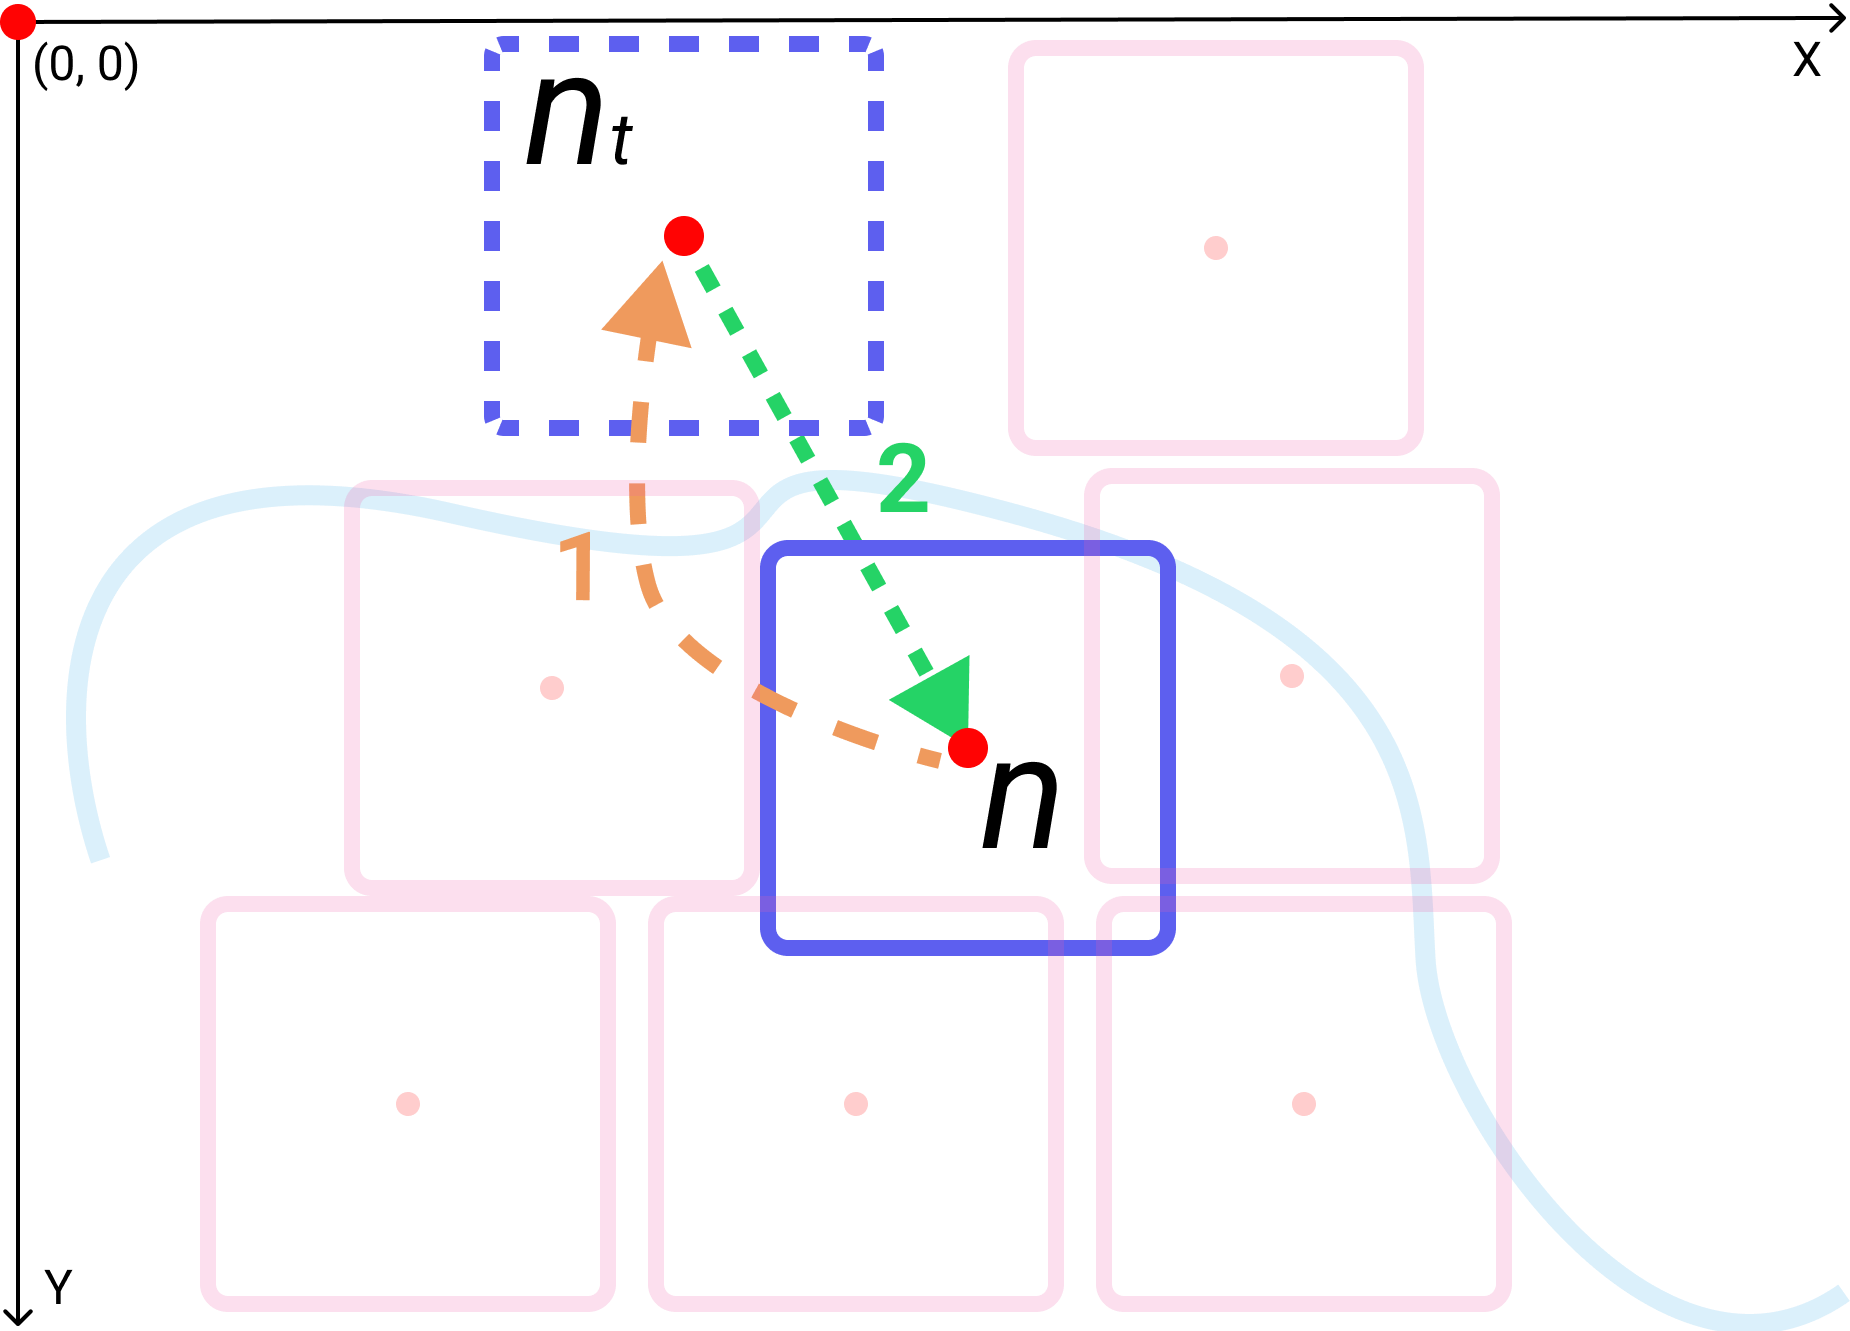
\includegraphics[width=\columnwidth]{figure/stalemate.png}
    \caption{A stalemate situation is when a node repeatedly translates between two positions (A and B) for more than $ stalemate $ iterations. }
    \label{fig:stalemate}
\end{figure}
}

{
\begin{figure}[tb!]
    \centering
    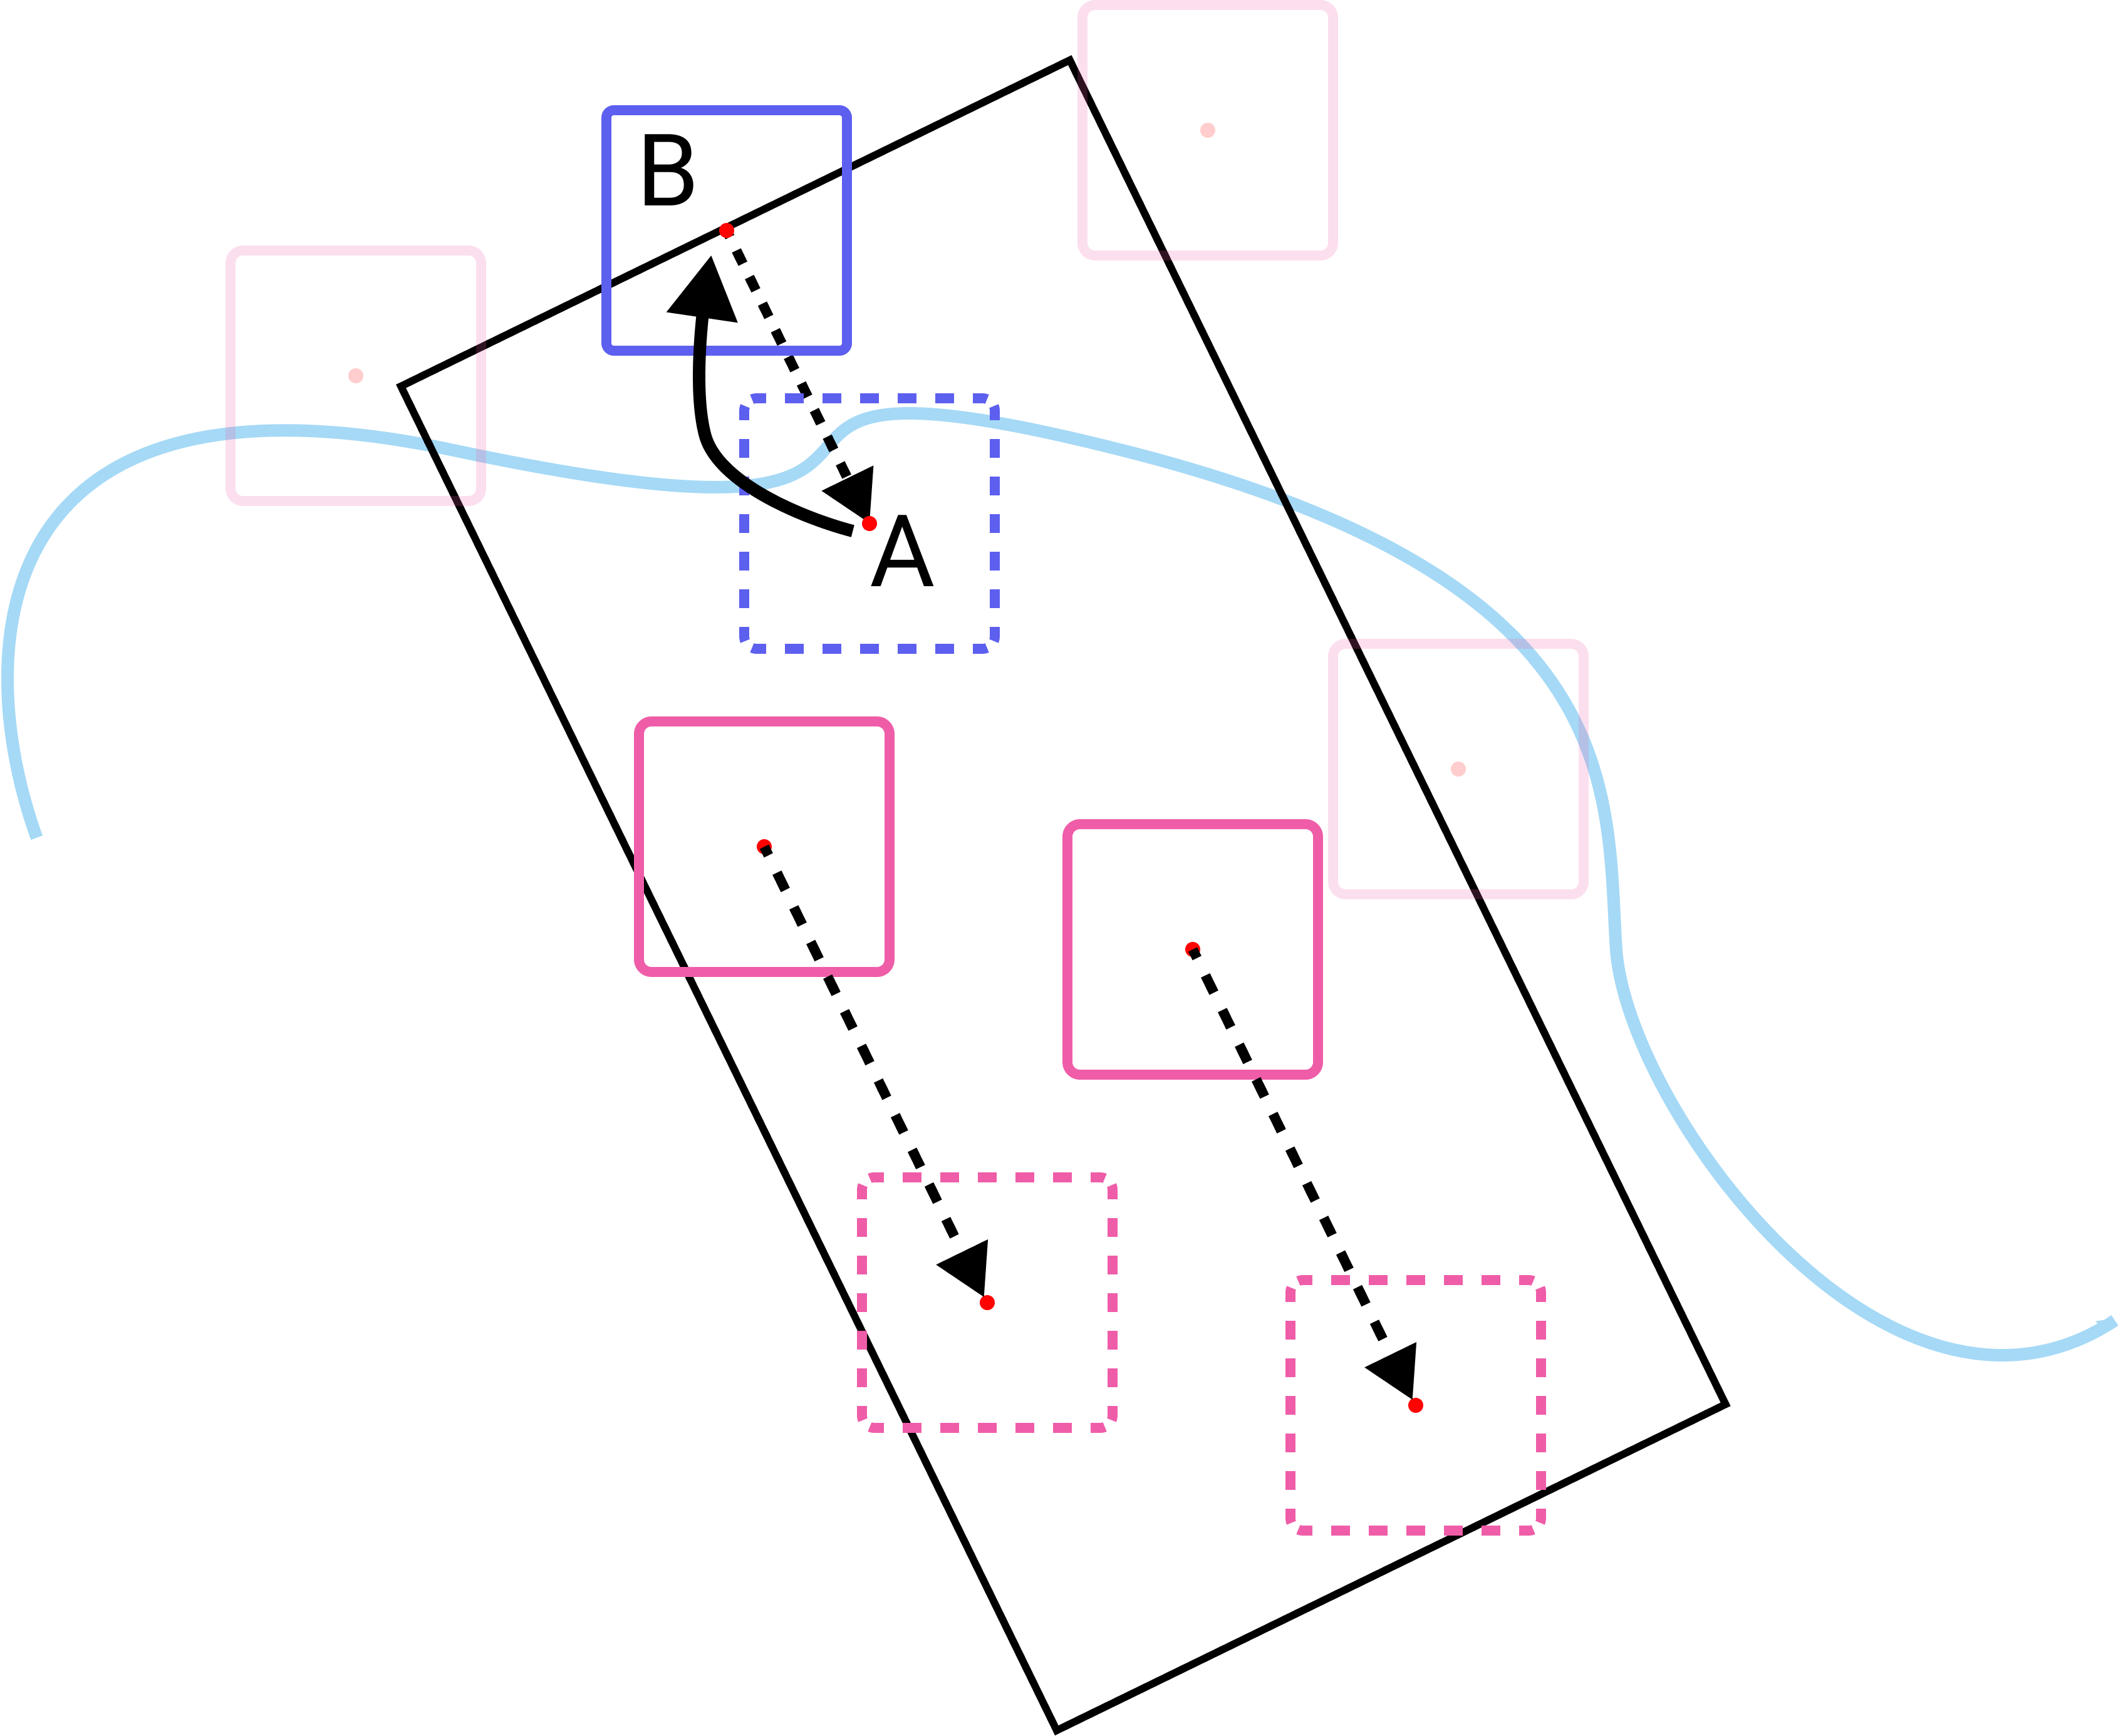
\includegraphics[width=\columnwidth]{figure/corridor.png}
    \caption{When a stalemate occurs, a corridor (black rectangular) is derived based on the current (A) and previous (B) positions of the node that crossed a river, as described in \algoref{alg:derive corridor}. All nodes within the corridor are moved by $ d $ units in the direction of $ \Vector{B}{A} $, e.g, A is moved to C. }
    \label{fig:corridor}
\end{figure}
}

% \begin{noindent}

\begin{algorithm}[tb!]
    \caption{Procedure to derive a corridor to translate enclosed nodes. We use an SVG canvas, where the point of origin (0,0) is located at the top left corner, with the x-axis extending to the right and the y-axis extending downwards.}\label{alg:derive corridor}

    \textbf{Input:} \\
    $ \node \gets $ the node used to derive the corridor \\

    \textbf{Global variables:} \\
    $ \nodeSize \gets $ the current size of all nodes \\
    $ \CorridorLength \gets $ the length of a corridor \\
    $ \CorridorWidth \gets $ the width of a corridor \\

    \textbf{Local variables:} \\
    $ \PointP \gets $ the point extending $ \Vector{\node.previous}{~\node} $ such that the length of $ \Vector{\node.previous}{~\PointP} $ is $ \CorridorLength $\\
    $ \EdgeParallelA, \EdgeParallelB \gets $ the edges parallel to $ \Vector{\node}{\PointP} $ \\
    $ corridor \gets $ a rectangular formed by $ \EdgeParallelA $ and $ \EdgeParallelB $ \\

    \begin{algorithmic}[1]
        \Procedure{DeriveCorridor}{$ \node $}
            \State TranslateNode ($ \node $)

            \State $ \PointP \gets $ \Call{DerivePoint}{$ \Vector{\node.previous}{~\node} $, $ \CorridorLength $}

            \State $ \EdgeParallelA \gets $ \Call{DeriveParallelEdge}{$ \Vector{\node.previous}{~\PointP} $, $ \frac{\CorridorWidth}{2} $}

            \State $ \EdgeParallelB \gets $ \Call{DeriveParallelEdge}{$ \Vector{\node.previous}{~\PointP} $, $ -\frac{\CorridorWidth}{2} $}

            \State $ corridor \gets
                \begin{bmatrix}
                    \EdgeParallelA.start &
                    \EdgeParallelA.end \\

                    \EdgeParallelB.start &
                    \EdgeParallelB.end \\
                \end{bmatrix} $

            \ForEach{$ \nodeInCorridorEach $ inside $ corridor $}
                \State $ \nodeInCorridorEachDx \gets \nodeInCorridorEach.x - \nodeInCorridorEach.previous.x $

                \State $ \nodeInCorridorEachDy \gets \nodeInCorridorEach.y - \nodeInCorridorEach.previous.y $

                \State $ hyp \gets \sqrt{(\nodeInCorridorEachDx)^2 +(\nodeInCorridorEachDy)^2} $

                \State $ \nodeInCorridorEach.next \gets $ \Call{DerivePoint}{$ \Vector{\nodeInCorridorEach.previous}{~\nodeInCorridorEach} $, $ hyp + s $}

                \State TranslateNode ($ \nodeInCorridorEach $, $ \nodeInCorridorEach.next $)

            \EndFor
        \EndProcedure
    \end{algorithmic}
\end{algorithm}

%\end{noindent}

% \begin{noindent}

    \begin{algorithm}[tb!]
        \caption{Procedure to derive a point based an edge and a distance.}\label{alg:derive corridor point}
        \textbf{Input:} \\
        $ \Edge \gets $ the edge used to derive the new point \\
        $ \Distance \gets $ the distance between $ \PointP $ and $ \Edge.start $ \\

        \textbf{Output:} \\
        A point, $ \PointP $, that is distance $ \Distance $ away from $ \Edge.start $. \\
    
        \textbf{Local variables:} \\
        $ \dx, \dy \gets $ the differences in $ x, y $ for $ \Edge.start $ and $ \Edge.end $ \\
    
        \begin{algorithmic}[1]
            \Procedure{DerivePoint}{$ \Edge $, $ \Distance $}
                \State $ \dx \gets \Edge.start.x - \Edge.end.x $
    
                \State $ \dy \gets \Edge.start.y - \Edge.end.y $
    
                \State $ \PointP.x \gets \frac{\dx}{\sqrt{\dx^2 + \dy^2}} \cdot \Distance $
    
                \State $ \PointP.y \gets \frac{\dy}{\sqrt{\dx^2 + \dy^2}} \cdot \Distance $
    
            \State \Return{$ \PointP $}
    
            \EndProcedure
    
        \end{algorithmic}
    \end{algorithm}
    
    %\end{noindent}


% \begin{noindent}

\begin{algorithm}[tb!]
    \caption{Procedure to derive an edge, $ \EdgeParallel $, that is parallel to $ \Edge $ with a distance of $ \Distance $.}\label{alg:derive corridor edge}

    \textbf{Input:} \\
    $ \Edge \gets $ the edge used to derive the parallel edge $ \EdgeParallel $ \\
    $ \Distance \gets $ the distance between $ \Edge $ and $ \EdgeParallel $ \\

    \textbf{Output:} \\
    An edge, $ \EdgeParallel $, that is parallel to $ \Edge $ with a distance of $ \Distance $. \\

    \textbf{Local variables:} \\
    $ \dx, \dy \gets $ the differences in $ x, y $ for $ \Edge.start $ and $ \Edge.end $ \\
    $ \Scale \gets $ the scale of $ \frac{\Distance}{\sqrt{\dx^2 + \dy^2}} $ \\

    \begin{algorithmic}[1]
        \Procedure{DeriveParallelEdge}{$ \Edge $, $ \Distance $}
            \State $ \dx \gets \Edge.start.x - \Edge.end.x $

            \State $ \dy \gets \Edge.start.y - \Edge.end.y $

            \State $ \Scale \gets \frac{\Distance}{\sqrt{\dx^2 + \dy^2}} $

            \State $ \EdgeParallel.start.x \gets \Scale \cdot -\dy + \Edge.start.x $

            \State $ \EdgeParallel.start.y \gets \Scale \cdot \dx + \Edge.start.y $

            \State $ \EdgeParallel.end.x \gets \Scale \cdot -\dy + \Edge.end.x $

            \State $ \EdgeParallel.end.y \gets \Scale \cdot \dx + \Edge.end.y $

        \State \Return{$ \EdgeParallel $}

        \EndProcedure

    \end{algorithmic}
\end{algorithm}

%\end{noindent}